\cotefile{91}
\scanpage{99}
% L1
\[
= \varinjlim_{\unsure{\mathfrak P|\mathcal P}}\ \varprojlim_j\
\deleted{\unsure{\operatorname{Hom}}}\prod_\alpha
\operatorname{Hom}(X_\alpha^{\mathfrak P},Y_j)
\]

\begin{center}\rule{1.4cm}{0.4pt}\end{center}

% L2--5; vertical pen stroke beside the heading and the opening of the sentence.
\noindent\llap{\raisebox{-1.1ex}{\rule{0.35pt}{2.4ex}}\hspace{.35em}}Ensembles quasi-schématiques.

Les ens quasi-schématiques de type fini sur un \deleted{\unsure{schéma}} ens quasi-schématique \uline{noethérien} forment une \uline{catégorie géométrique} (?)
% archive sheet number: 98
\scanpage{100}
\mspage{- 12 -}\hfill n\textsuperscript{o} 285

% L1
se borner au cas où $I$ est un intervalle de \hspace{1.2em}, et comme la proposition
% L2
est triviale si $I$ est fini, on peut supposer $I=\mathbb{N}$. Soit $x_p\handwritten{\in}G_p$ ;
% L3
l'hypothèse permet de définir par récurrence sur $n\handwritten{\geqslant}p$ une suite $(x_n)_{n\handwritten{\geqslant}p}$
% L4
satisfaisant aux conditions $x_n\handwritten{\in}G_n$, $f_{n,n+1}(x_{n+1})=x_n$ ; il est clair
% L5
alors que si on pose, pour $m\handwritten{<}p$, $x_m=f_{mp}(x_p)$ la suite $(x_n)_{n\handwritten{\geqslant}0}=x$
% L6
appartient à $G$ et que $f_p(x)=x_p$, d'où la proposition.

% L7
PROPOSITION 23 - \uline{Les notations étant celles du cor}.1 \uline{de la prop.}20,
% L8
\uline{on suppose en outre que pour tout} $\alpha\handwritten{\in}I$, \uline{l'application canonique} $\varphi_\alpha$ \uline{de} $A$
% L9
\uline{dans} $A_\alpha$ \uline{soit surjective}. \uline{Alors}, \uline{si pour tout} $\alpha\handwritten{\in}I$ $g_\alpha(A_\alpha)$ \uline{est dense}
% L10
\uline{dans} $B_\alpha$, $g(A)$ \uline{est dense dans} $B$.

% L11
En effet, il suffit de montrer que, pour tout $\alpha\handwritten{\in}I$ et tout ensemble
% L12
ouvert non vide $U_\alpha$ dans $B_\alpha$, il existe $x\handwritten{\in}A$ tel que $\handwritten{\psi}_\alpha(g(x))\handwritten{\in}U_\alpha$ (en
% L13
désignant par $\handwritten{\psi}_\alpha$ l'application canonique de $B$ dans $B_\alpha$). Mais par hypothèse
% L14
il existe $x_\alpha\handwritten{\in}A_\alpha$ tel que $g_\alpha(x_\alpha)\handwritten{\in}U_\alpha$, et il existe $x\handwritten{\in}A$ tel que
% L15
$\varphi_\alpha(x)=x_\alpha$ ; comme $\handwritten{\psi}_\alpha(g(x))=g_\alpha(\varphi_\alpha(x))$, cet élément répond à la question

% L16
PROPOSITION 24 - \uline{Soient} $(G_\alpha,f_{\alpha\handwritten{\beta}})$ \uline{un système projectif de groupes}
% L17
\uline{topologiques}, $G=\underset{\handwritten{\longleftarrow}}{\lim}\,G_\alpha$, $f_\alpha$ \uline{l'application canonique de} $G$ \uline{dans} $G_\alpha$. \uline{On}
% L18
\uline{suppose que} : 1\textsuperscript{o}) \uline{pour tout} $\alpha\handwritten{\in}I$, $f_\alpha$ \uline{est surjective} ; 2\textsuperscript{o}) \uline{pour tout}
% L19
\uline{couple d'indices tel que} $\alpha\handwritten{\leqslant}\handwritten{\beta}$, $f_{\alpha\handwritten{\beta}}$ \uline{est un homomorphisme de} $G_{\handwritten{\beta}}\unsure{{}^{\cdot\cdot}|{:}}$ \uline{sur}
% L20
$G_\alpha$. \uline{Dans ces conditions}, $f_\alpha$ \uline{est un homomorphisme de} $G$ \uline{sur} $G_\alpha$.

% L21
En effet, soit $V$ un voisinage quelconque de $e$ dans $G$. Il existe un
% L22
indice $\handwritten{\beta}\handwritten{\geqslant}\alpha$ et un voisinage $V_{\handwritten{\beta}}$ de $e_{\handwritten{\beta}}$ dans $G_{\handwritten{\beta}}$ tel que $W=f^{-1}_{\handwritten{\beta}}(V_{\handwritten{\beta}})$
% L23
soit un voisinage de $e$ contenu dans $V$. Comme $f_{\handwritten{\beta}}$ est surjective, on a
% L24
$V_{\handwritten{\beta}}=f_{\handwritten{\beta}}(W)$, et comme $f_{\alpha\handwritten{\beta}}$ est un homomorphisme surjectif, $f_{\alpha\handwritten{\beta}}(V_{\handwritten{\beta}})$
% L25
est un voisinage de $e_{\handwritten{\unsure{\delta|\alpha}}}$ dans $G_\alpha$ ; mais on a $f_\alpha(W)=f_{\alpha\handwritten{\beta}}(f_{\handwritten{\beta}}(W))=$
% L26
$=f_{\alpha\handwritten{\beta}}(V_{\handwritten{\beta}})$ d'où la proposition (th.1).

% L27
Soit $N_\alpha$ le noyau de $f_\alpha$ ; les $N_\alpha$ constituent une base de filtre, formée
% archive sheet number: 99
\scanpage{101}
% L1
\deleted{\unsure{Ens de schémas sur $k$|Pseudo-schémas sur $k$}}

% L2
\diagram{\begin{tikzcd}[ampersand replacement=\&,column sep=large]
(\text{Ens. schématiques }\unsure{\}}\,\text{sur }k)
\arrow[r,swap,"\text{\unsure{pl.|pl\textsuperscript{t}.} fidèle}"] \&
\underline{\operatorname{Hom}}((\text{Ens schém.}/k),(\text{Ens}))
\end{tikzcd}}

% L3
\diagram{\begin{tikzcd}[ampersand replacement=\&,column sep=small]
\& X \& \& \\
S\arrow[ur,dashed,"\unsure{i}"] \& \& S'\arrow[ul]\arrow[ll] \& S''\arrow[l,shift left=.55ex]\arrow[l,shift right=.55ex]
\end{tikzcd}}

% L4
\deleted{\uline{application surjective}} \qquad \uline{morphisme fid. plat}

% L5
\uline{Tout épimorphisme est un morphisme de descente}

% L6--9; braces group 1--4, square brackets group 1--2 and 3--4.
\[
\left\{\begin{array}{l}
\left[\begin{array}{ll}
1) & \text{Existence de }\varprojlim\text{ finies}\\
2) & \text{Existence du quotient par un \unsure{graphe|couple|groupoïde} d'équivalence}
\end{array}\right.\\[3pt]
\left[\begin{array}{ll}
3) & \text{Tout épim est effectif}\\
4) & \text{Tout épim est universel}
\end{array}\right.
\end{array}\right.
\]
\margin{[\unsure{d'où|donc|dans} ça marche pour \unsure{prégraphes|prégroupes|présystèmes|groupoïdes} d'équivalence\ldots]}
% slanted; a long curved stroke goes down the right edge to the question mark beside 4').

% L10
\deleted{5) Tout morphisme se factorise par un produit \unsure{du|dans} [\unsure{épim, un mono}]}

% L11; encircling and crossing strokes over the right branch.
\diagram{\begin{tikzcd}[ampersand replacement=\&,column sep=small,row sep=small,execute at end picture={\draw[thin] ($(\tikzcdmatrixname-1-2.west)+(-.15,0)$) .. controls +(0,.8) and +(0.7,.6) .. ($(\tikzcdmatrixname-1-5.east)+(.18,.06)$) .. controls +(.5,-1.0) and +(.3,-.4) .. ($(\tikzcdmatrixname-2-5.south)+(-.4,-.05)$) .. controls +(-1,.10) and +(0,-.50) .. cycle; \draw[thin] (\tikzcdmatrixname-1-3.east) .. controls +(0,-.5) and +(-.2,-.4) .. (\tikzcdmatrixname-1-4.south) .. controls +(.2,.8) and +(-.15,.5) .. (\tikzcdmatrixname-2-5.west) .. controls +(.6,.45) and +(-.5,.08) .. (\tikzcdmatrixname-2-5.east);}]
\deleted{\unsure{E}}\arrow[r] \& \deleted{\unsure{1}} \&
\deleted{X\times_Y X}\arrow[r,shift left=.55ex]\arrow[r,shift right=.55ex] \&
\deleted{X}\arrow[r]\arrow[dr] \& \deleted{Y}\\
\& \& \& \& \deleted{\unsure{Y'\mathrm{Im}|Y'/\mathrm{Im}|X/\mathrm{Rel}}}
\end{tikzcd}}

% L12--15
\[
\left\{\begin{array}{l}
\left[\begin{array}{ll}
1') & \text{Existence de }\varinjlim\text{ finies}\\
2') & \text{Existence du \unsure{coquotient|conoyau} par un \unsure{cographe|cocouple|couple} d'équivalence}
\end{array}\right.\\[3pt]
\left[\begin{array}{ll}
3') & \text{Tout. mon est effectif}\\
4') & \text{\unsure{Cochangement|Co-changement|Changement} de base dans un monomorphisme}
\end{array}\right.
\end{array}\right.
\]
\margin{?}

% L16
\uline{Axiome géométrique} \qquad $X\times\coprod Y_i\simeq\coprod_i X\times Y_i$

% L17--18
[\unsure{ou aussi|en somme} : changt de base commute aux sommes, -- donc aux $\uline{\lim}$ finies ???]

% L19
$R\to S$
\figure{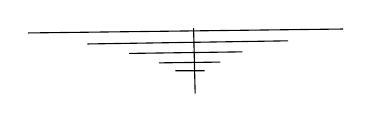
\begin{tikzpicture}[x=1cm,y=1cm]
\draw (-2,.40)--(2,.45) (-1.25,.26)--(1.30,.30) (-.72,.14)--(.72,.16) (-.34,.02)--(.44,.03) (-.13,-.08)--(.24,-.08) (.10,.46)--(.12,-.37);
\end{tikzpicture}}
% archive sheet number: 100
\scanpage{102}
\mspage{- 10 -}\hfill n\textsuperscript{o} 285

% L1
topologiques $(G_\alpha)$ et la famille d'applications $(j_\alpha\handwritten{\circ}g_\alpha)$, en désignant
% L2
par $g_\alpha$ l'application canonique de $H$ dans $H_\alpha$. Comme $j_\alpha\handwritten{\circ}g_\alpha=f_\alpha\handwritten{\circ}j$,
% L3
le même critère de transitivité prouve que $j$ est un isomorphisme de $H$
% L4
sur le sous-groupe $j(H)$. En outre, $j(H)$ est l'intersection, dans le groupe
% L5
produit $F=\handwritten{\prod}_{\alpha\handwritten{\in}I}G_\alpha$, de $G$ et du sous-groupe $\handwritten{\prod}_{\alpha\handwritten{\in}I}H_\alpha$ d'où la dernière
% L6
assertion du corollaire.

% L7
Lorsque les hypothèses du cor.2 sont satisfaites, on dit que $(H_\alpha)$ est
% L8
un \uline{système projectif de sous-groupes} correspondant au système projectif
% L9--10
de groupes $(G_\alpha)$, et on identifie d'ordinaire $H$ et $j(H)$ au moyen de l'injection $j$.

% L11
Soit $K$ un sous-groupe de $G=\underset{\handwritten{\longleftarrow}}{\lim}\,G_\alpha$, et posons $K_\alpha=f_\alpha(K)$ ; il est
% L12
immédiat que $(K_\alpha)$ est un système projectif de sous-groupes dont la
% L13
\margin{\handwritten{\unsure{2|Z}}}limite projective $H$ s'identifie à un sous-groupe de $G$. Il est clair
% L14
en outre que $H\handwritten{\supset}K$ et on voit aussitôt que $K$ est dense dans $H$
% L15
(cf. prop.23) ; mais en général on aura $H\ne K$ (exerc. voir \handwritten{\S}3,
% L16
cor.1 de la prop.18).

% L17
\uline{Corollaire} 3 - \uline{Les hypothèses et notations étant celles du cor}.1,
% L18--19
\uline{soit} $N_\alpha$ \uline{le noyau de} $g_\alpha$ ; \uline{alors} $(N_\alpha)$ \uline{est un système projectif de sous-groupes distingués}, \uline{dont la limite projective est} \uline{le noyau de} $g=\underset{\handwritten{\longleftarrow}}{\lim}\,g_\alpha$

% L20
La relation $g_\alpha\handwritten{\circ}\varphi_{\alpha\handwritten{\beta}}=\handwritten{\psi}_{\alpha\handwritten{\beta}}\handwritten{\circ}g_{\handwritten{\beta}}$ pour $\alpha\handwritten{\leqslant}\handwritten{\beta}$ montre aussitôt que
% L21
$(N_\alpha)$ est un système projectif. En outre, si $\varphi_\alpha$ (resp. $\handwritten{\psi}_\alpha$) est l'application
% L22
canonique de $A$ dans $A_\alpha$ (resp. de $B$ dans $B_\alpha$), la relation $\handwritten{\psi}_\alpha(g(x))=$
% L23
$=g_\alpha(\varphi_\alpha(x))$ pour $x\handwritten{\in}A$ montre que si $x\handwritten{\in}N=\underset{\handwritten{\longleftarrow}}{\lim}\,N_\alpha$, on a $\handwritten{\psi}_\alpha(g(x))=e$
% L24
pour tout $\alpha\handwritten{\in}I$, donc $g(x)=e$, et réciproquement cette dernière relation
% L25
entraîne $\varphi_\alpha(x)\handwritten{\in}N_\alpha$ pour tout $\alpha\handwritten{\in}I$, donc $x\handwritten{\in}N$. Ce raisonnement montre
% L26
en outre que $N$ est \uline{l'intersection des sous-groupes} $\varphi^{-1}_\alpha(N_\alpha)$ (qui forment
% L27
une base de filtre, comme on le vérifie aussitôt ).
% archive sheet number: 101
\scanpage{104}
% L1--6
\uline{Définition} 1 Soit $X$ un espace topologique. On appelle topologie constructible de $X$, \deleted{\unsure{et on}} la topologie dont les ouverts sont les réunions quelconques de parties loc. constructibles [donc une base d'ouverts \unsure{fournie|formée} par les parties loc constructibles,]. Parties \unsure{antitypiques|antypiques|indéfiques|analytiques} $=$ fermés de $X^{\mathrm{cons}}$ $=$ intersections des parties loc constructibles.

% L7--8; several separate vertical emphasis strokes at the left of the proposition.
\margin{\deleted{\illegible{2}}}
% slanted
\uline{Prop 1} Supposons que \deleted{tout point de} $X$ admette une base \inserted{$(U_i)_{i\in I}$} formée d'\deleted{ouverts} rétrocompacts. Alors

% L9
(0) les parties constructibles de $X$ forment une base d'ouverts de $X^{\mathrm{cons}}$

% L10--11
(i) La topologie constructible de $X$ est plus fine que la topologie donnée, \unsure{i.e.} $X^{\mathrm{cons}}\longrightarrow X$ est continue.

% L12--13
(ii) \deleted{\unsure{Si de|Supposons}} \inserted{Si} $X$ satisfait de plus $T_0$, alors $X^{\mathrm{cons}}$ est séparé [et $=$ tot. discontinu] et réciproquement

% L14--17
(iii) Si \deleted{$\unsure{U|E}$} $E$ est une \deleted{ouvert de $X$, la topologie} \inserted{partie constructible de $X$,} munie de la topologie induite $T_E$, alors la topologie constructible $T_E^{\mathrm{cons}}$ associée : $T_E$ est induite par $T^{\mathrm{cons}}$ sur $E$.

% L18--19
(0) Car \deleted{\unsure{tt}} un loc. constructible $E$ est réunion des $U_i\cap E$, qui sont constructibles dans $X$ par $\unsure{0_{\mathrm I}|0_{\mathrm{III}}}$ 9.1.8.

% L20--26
(i) Résulte du fait que les $U_i$ sont \inserted{[loc.]} constructibles, donc ouverts pour $T_{\unsure{E|X}}^{\mathrm{cons}}$. Pour (ii), \deleted{\unsure{soit|soient}}, $x,y\in X$, il existe \unsure{un des deux|l'un des deux}, disons $x$, et un voisinage ouvert $U\ni x$, $U\not\ni y$. On peut grâce à l'hyp supposer $U$ rétrocomp\unsure{act}, donc [loc.] constructible, et $X-U=V$ l'est \inserted{alors} également, alors $U\cap V=\emptyset$, $U\cup V=X$, $U\ni x$, $V\ni y$, $U,V$ ouverts pour $T_E$.

% L27--30
Pour (iii), on note que la topologie induite par $T_{\unsure{X|E}}^{\mathrm{cons}}$ sur $E$ a comme base d'ouverts les $E\cap F$, $F$ \deleted{\unsure{un|const.}} \inserted{loc.} constructible dans $X$, ce sont exactement les $G\subset E$ loc. constructibles dans $E$,
% archive sheet number: 103
\scanpage{105}
% L1
grâce au

% L2--3
\uline{Lemme} \quad a) Soit \deleted{$\unsure{E}$} $F$ (loc.) constructible dans $X$, \inserted{$E$ loc. const.} alors $F\cap E$ est (loc) constructible dans $E$

% L4--5
b) Soit \deleted{$\unsure{E}$} $F\subset E$, \inserted{avec $E$ (loc) constructible} alors $F$ est (loc.) constr. dans $E$ ssi il l'est dans $X$.

% L6--8
Dém. Pour a), on \unsure{montre|note} que si $F$ est ouvert rétrocompact dans $X$, alors $F\cap E$ est rétrocompact dans $E$, grâce au fait que tt ouvert \unsure{qu. cpt} $U$ de $E$ est
\diagram{\begin{tikzcd}[ampersand replacement=\&,row sep=small,column sep=small]
E\arrow[d,"f"] \& f^{-1}(F)\cap U\\
X \& F
\end{tikzcd}}
% L9--13
induit par un ouvert $V$ de $X$, qu'on peut si on veut [grâce à l'hyp \unsure{particulière|préliminaire} de la prop] supposer qu. cpt, d'où $f^{-1}(F)\cap U=f^{-1}(F\cap V)=$ image inverse d'un qu. cpt, qui est qu. cpt car $E$ est rétrocompact dans $X$, \deleted{\unsure{Donc|Dans}} \inserted{par $\unsure{0_{\mathrm{III}}|0_{\mathrm I}}$ 9.1.13.} Le cas ``localement''
% L14--16
en résulte aussitôt, utilisant le fait que $E$ induit un $E\cap U$ constructible dans \deleted{tt} $U$ ouvert\deleted{\unsure{e}}.

% L17--20
Pour b), on suppose $F\subset E$ constructible dans \uline{$E$} \inserted{\unsure{loc. ctr.|constr.}}, prouvons que $F$ l'est dans $X$. On peut supposer $F$ \deleted{\unsure{ouvert}} \deleted{fermé} \inserted{ouvert} dans $E$, rétrocompact dans $E$, \deleted{et} \inserted{\unsure{puis : et|puis : a)} cas} $E=U\cap \complement V$, $U$ et $V$ rétrocomp. \unsure{ds} dans $X$ \inserted{qui sont constructibles}
% L21--24
[car $E=\bigcup E_i$ réunion finie de tels, les \deleted{$F\cap E_i$ sont} dans \uline{$E$} par a), donc $E_i\cap F$ constr. dans $E_i$ par a), et on est ramené à prouver qu'ils sont constructibles dans $X$, puisque $F=\bigcup E_i\cap F$.
\margin{$0_{\unsure{\mathrm{II}|\mathrm{III}}}$ 9.1.8 \unsure{(i) b(ii)|(i) (ii)|(i) bis|(i)$\Rightarrow$(ii)}}
% L25--26
\deleted{\unsure{De sorte} $F$ \unsure{étant ouvert dans $E$, on} $F=$ \unsure{l'est-il|$E\cap W$}, \unsure{à fortiori dans} $X$, \unsure{donc}} \inserted{Remplaçant $X$ par $U$, on peut grâce à \deleted{\unsure{une hyp}} se borner au cas $X=U$ [$E$ étant constr. dans $U$\inserted{par \unsure{(i)|(ii)}}, $F$ \deleted{\unsure{donc|alors}} le sera dans $U$, donc dans $X$]}
% Large unlettered pen stroke in the lower left margin.
\figure{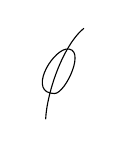
\begin{tikzpicture}[scale=.34]\draw (0,-1.6) .. controls (.05,-.6) and (.64,1.15) .. (1.43,1.8); \draw (.33,-.64) .. controls (-.65,-.63) and (.17,.89) .. (.76,1.02) .. controls (1.56,1.12) and (.75,-.64) .. (.33,-.64);\end{tikzpicture}}
% archive sheet number: 104
\scanpage{106}
% L1--5
Donc on peut supposer $E=\complement V$, $V$ \deleted{\unsure{ét|rét.}} ouvert rétrocompact, \deleted{et par suite on aura $\unsure{E-F=F=\complement}$ \unsure{un ouv.}} Il suffit de prouver \inserted{le fermé} $E-F$ constr. dans $X$, i.e. $X-(E-F)=V\cup F$ rétrocompact dans $X$, ce qui est le cas car $V$ et $F$ le sont évidemment \unsure{\ldots}

% Small sketch in the left margin at L3--5.
\figure{\begin{tikzpicture}[scale=.68]
\draw (.1,0)--(.82,2.45); \draw (.08,.28)--(.21,.24) (.63,2.12)--(.75,2.08);
\node at (.47,1.13) {$F$}; \node[above right] at (.8,2.4) {$\complement V$};
\end{tikzpicture}}

% L6
Le cas ``local'' résulte aussitôt du cas global.

% L7--11
\uline{Corollaire} 1 Supposons que de plus, tte partie $U_i$ soit \uline{quasi compacte} \deleted{\unsure{[alors ce}} \uline{pour la topologie constructible} [donc aussi \deleted{pour la top.} compacte pour la top constructible, dans le cas où \deleted{la top} $X$ satisfait (T$_0$)], \inserted{i.e. satisfasse à la condition : \unsure{théorème 1|th. 1}} Alors

\margin{N.B. les hypothèses faites signifient que tte partie fermée \unsure{irrid.|irréd.} de $X$ admet un \deleted{\unsure{pt}} pt générique (unique si (T$_0$) est satisfait \unsure{\ldots})}
% slanted

% L12--14
(iv) Les $U_i^{\mathrm{cons}}$ sont quasi-compacts, \deleted{et \unsure{tout} \inserted{et $X$} \unsure{est} ouvert quasi-compact \unsure{est une base formée d'ouverts} [donc $X$ admet une base formée d'ouverts]}

% L15--18
(v) Soit $E$ une partie \deleted{loc. constructible de} \inserted{fermée de} $X^{\mathrm{cons}}$ [p. ex. une partie loc. constructible \deleted{\unsure{]}} de $X$] alors $E$ \deleted{compact} quasi-compact \inserted{[resp. cpt]} dans $X^{\mathrm{cons}}$ $\Longleftrightarrow$ $E$ quasi-compact dans $X$ $\Longleftrightarrow$ $E\subset$ réunion finie des $U_i$.

% L19--20
(vi) Pour que $X^{\mathrm{cons}}$ soit loc. cpt [cpt] il f. et s. que $X$ satisfasse (T$_0$) [\unsure{resp.} (T$_0$) et soit qu. cpt].

% L21--26
(iv) Résulte de (i) trivialement. Evident $E^{\mathrm{cons}}$ qu. cpt $\Rightarrow$ $E$ qu. cpt en vertu de (i) $\Rightarrow$ $E\subset$ réunion finie \inserted{$V$} des $U_i$ par définition de qu. cpt, donc $E$ fermé dans $V^{\mathrm{cons}}$ [pour la top. induite par $X^{\mathrm{cons}}$] qui est aussi $\bigcup U_i^{\mathrm{cons}}$, et les $U_i^{\mathrm{cons}}$ étant qu. cpts, il s'ensuit que $E$ l'est, O.K. \quad (vi) En résulte \unsure{hic et nunc|l'assertion|trivialement}
% archive sheet number: 105
\scanpage{107}
% L1--5
\uline{Corollaire} 2 \deleted{Sous les conditions du corollaire 1,} Supposons $X$ \deleted{de plus} quasi compact \inserted{et (T$_0$)}, et que \deleted{tte partie} $X$ ait une base formée d'ouverts \deleted{\unsure{qu. cpts|qu.-cpts}} rétrocompacts, qui sont qu. cpts pour la topologie constructible. Soit $E$ une partie de $X$. Conditions équivalentes

% L6--7
a) $E$ est fermé pour la top. constructible [i.e. est intersection \deleted{pour la} de parties constructibles]

% L8--11
b) $E$ est compact pour la top. constructible, i.e. pour tte famille de parties constructibles $(E_i)_{i\in I}$ de $X$, telle que $E\subset\bigcup_{i\in I}E_i$, il existe une sous-famille finie $J\subset I$, telle que $E\subset\bigcup_{i\in J}E_i$.

\margin{-- \unsure{généralt|général}, \uline{partie \unsure{antitypique|antypique|atypique|analytique}} $=$ \uline{intersection de loclt constructibles} Nature locale de la notion ??}
% slanted

% L12
\deleted{$X$ \unsure{est}} En effet, $X^{\mathrm{cons}}$ est compact, donc a) $\Longleftrightarrow$ b).

% L13--16
On dit parfois \inserted{alors} que \deleted{$X$} $E$ est une \uline{partie antitypique de} $X$. On peut donner un \unsure{énoncé} analogue si $X$ n'est plus supposé qu cpt [mais satisfaisant aux autres hyp]

% L17--20
\[
\begin{aligned}
& E\ \text{fermé \inserted{dans $X^{\mathrm{cons}}$} [i.e. intersection de parties loc. constructibles]}\\
& \Updownarrow\\
& E\ \text{loc cpt pour la top. constructible i.e. pour tt}\\
& \text{\deleted{partie \unsure{ouverte}} }U_i,\quad E\cap \deleted{\unsure{E|X}}U_i\ \text{satisfait la condition b}\\
& \text{ci-dessus dans } U_i .
\end{aligned}
\]

% L21--25
\uline{Corollaire} 3 Sous les conditions du corollaire 2, Conditions équivalentes

a) $E$ et $X-E$ sont antitypiques

b) $E$ est \deleted{constructible} ouvert et fermé dans $X^{\mathrm{cons}}$

c) $E$ est constructible.
% archive sheet number: 106
\scanpage{108}
% L1--6
$c\Rightarrow a)\Longleftrightarrow b)$ trivial, pour la réciproque $a\Rightarrow c$, notons que $E$ et $X-E=F$ étant ouverts dans $X^{\mathrm{cons}}$, sont réunions \deleted{\unsure{d'ouverts}} \deleted{d'ens} filtrées d'ens constructibles $E_i$ respt. $F_j$, donc $X$ est réunion filtrante des $E_i\cup F_j$, donc est égal à l'un des $E_i\cup F_j$, d'où $E=E_i$, \deleted{$\unsure{F=F_j}$} $F=F_j$ pour ces $i,j$, donc $E_i,F_j$ constructibles

% L7--10
\uline{Proposition 2} Soit $f:X\longrightarrow Y$ une application continue d'espaces topologiques, telle que \deleted{\unsure{l'i.}} pour tt couple d'ouverts $V\subset U\subset Y$, \deleted{rétrocompact dans $Y$} \inserted{$V$ rétrocompact dans $U$,} $f^{-1}(\deleted{U}V)$ soit rétrocompact dans $\deleted{X}f^{-1}(U)$. Alors
\margin{Hyp. tjrs vérifiée pour un morphisme de préschémas}
% slanted

% L11
\deleted{(i) Pour tt ouvert $Y'$ de $Y$, posons $X'=f^{-1}(Y')$, $f':X'\longrightarrow Y'$ satisfait la \unsure{même} hyp. que $f$.}

% L12--14
\deleted{\unsure{(ii)}} (i) Pour tte partie constructible [loc. constructible] \deleted{\unsure{ouv}} \deleted{$U$} $E$ de $Y$, $f^{-1}(\deleted{U}E)$ est une partie constructible [loc constructible].

% L15--17
(ii) $f$ est continue de $X^{\mathrm{cons}}$ dans $Y^{\mathrm{cons}}$, i.e. l'image inverse d'une partie \inserted{\deleted{loc.}} \unsure{antitypique|antypique|atypique|analytique} de $Y$ est une partie \inserted{\deleted{loc.}} antitypique de $X$.

% L18--24
\margin{$Y'\subset Y$}
\deleted{\unsure{(a)}} (i) est trivial pour ``constructible''. Pour loc. constructible, on note qu'on \unsure{aura|a un} $Y=\bigcup Y_i$, les $Y_i$ ouverts, les $E_i=E\cap Y_i$ constructibles \inserted{dans $Y_i$}, soit $X_i=f^{-1}(Y_i)$, \inserted{$f_i:X_i\to Y_i$ induit,} il suffit de prouver que $f_i^{-1}(E_i)$ soit constructible dans $X_i$, donc de prouver que \inserted{$f_i$} $X_i\to Y_i$ satisfait l'hyp. de $f:X\longrightarrow Y$, \deleted{soit} O.K.

% L25
(ii) Résulte trivialt de (i).
% archive sheet number: 107
\scanpage{109}
% L1--8; oblique cancellation strokes through the entire first corollary.
\deleted{\uline{Corollaire} 1 Supposons que dans $X$ et $Y$, \deleted{tt pt} \unsure{admettant|admettent} une \deleted{\unsure{application fermée est de même}} \inserted{base d'ouverts \inserted{$X_i$ resp. $Y_j$} rétrocompacts quasi-compacts.} Alors l'hyp préliminaire de la prop. équivaut aussi à dire que pour tt ouvert \deleted{\unsure{qu. cpt}} $Y_j$, $f^{-1}(Y_j)$ est rétrocompact dans $X$, ou encore que pour tt \deleted{ouvert} ouvert $Y'$ \deleted{\unsure{qu. cpt dans}} \inserted{rétrocompact \deleted{\unsure{(ou rétrocompact)}}} $Y$, $X'=f^{-1}(Y')$ est \deleted{qu. cpt} rétrocompact dans $X$, ou encore que les $X_i\cap f^{-1}(Y_j)$ sont qu. cpts.}

% L9--13
[ \uline{Prop.} Soit $X$ un espace topologique, ayant une base d'ouverts $U_i$ qui sont quasi-compacts. Alors pour tte \deleted{partie $E$ de $X$, et \unsure{ouvert|toute}} application continue $f:X'\to X$, il revient au $=$ de dire que $f$ est qu. cpt, ou que les $f^{-1}(U_i)$ sont qu. cpts.

% L14--16
Donc si $X'\subset X$ sous-espace top., $X'$ est rétrocompact dans $X$ ssi les $X'\cap U_i$ sont qu. cpts.

% L17--19
\uline{Cor.} \deleted{Soit Supposons de \uline{plus}} \inserted{Pour que} les $U_i$ rétrocompacts dans $X$, \deleted{Alors} \inserted{il f. et s. que} \uuline{tte} partie quasi-compacte ouverte de $X$ soit rétrocompacte dans $X$.

% L20--25
\uline{Cor} S'il en est ainsi, pour une \deleted{\unsure{m}} application continue $f:X'\to X$ il revient au $=$ de dire \deleted{\unsure{que les}} (a) pour tt \inserted{ouvert} $U\subset X$ qui est rétrocompact, $f^{-1}(U)$ est rétrocompact, (b) Pour tt $U_i$, $f^{-1}(U_i)$ est rétrocompact dans $X'$, (c) [Si $X'$ a une base d'ouverts \deleted{\unsure{quasi rétrocompacts|quasicompacts}} $U'_j$] les $f^{-1}(U_i)\cap U'_j$ sont \deleted{rétro} quasi cpts.]

\margin{\deleted{\uline{Cor} Si $f$ \inserted{$:X'\to X$} est qu. cpt, et \unsure{dans $X'$ ttes les parties}}}
% slanted

% L22--27, small proof at lower left, continuing across the foot.
\margin{$b\Rightarrow a$, En effet, \inserted{$U\subset X$ ouv. rétrocomp., si $U'\subset X'$ ouv. qu. cpt} $f^{-1}(U)\cap V'$ \deleted{$=f^{-1}(U)\cap \unsure{f^{-1}}\cap$} $\subset f^{-1}(f(\unsure{U'|V'}))$, et $f(V')$ étant qu. cpt, est contenu dans une réunion \uline{finie} de $U_i$, $i\in J$, donc $f^{-1}(U)\cap V'=f^{-1}(\bigcup_{i\in J} U\cap U_i)\cap V'$ Or chaque $U\cap U_i$ est réunion \uline{finie} \unsure{d'ens|d'une|d'un} $\unsure{U_j|U_l}$}
% archive sheet number: 108
\scanpage{110}
% L1--4
\uline{Corollaire} 1 Supposons que $X$, \deleted{\unsure{soient des}} \inserted{$Y$ soient} des espaces (T$_0$), \deleted{schématiques \unsure{où|qui}} admettant des bases d'ouverts formées d'ens \deleted{quasi-compacts} rétrocompacts et qu. cpts pour la top. constructible [donc compacts pour la dite], \deleted{et que} \inserted{Conditions équivalentes :}

% L5
a) $f:X\longrightarrow Y$ \deleted{soit une telle que} \inserted{est} quasi compacte

% L6--9
\deleted{[par exemple $X$ Alors} b) $f^{\mathrm{cons}}$ est une \deleted{\unsure{application}} application propre d'espaces loc. cpts, \deleted{\unsure{ceci signifie|i.e.} $f$ [\unsure{et ses}] \unsure{parties de} $f$} \deleted{[et \inserted{alors $f$} transforme parties \unsure{antitypiques|antypiques|atypiques|analytiques} en parties antitypiques}

\inserted{c) $f$ transforme parties antitypiques en parties antitypiques, et les fibres de $f$ sont quasi-compactes [\unsure{appliq. de|appl. :} Bourbaki, Top \deleted{\unsure{II}} I, 10, 2, th. \uline{1}]}
% slanted

% L9--12
[N.B. $f$ en général ne transforme pas parties constructibles en parties constructibles, \deleted{et bien mieux on peut faire varier par \unsure{ouverts, idéal} ne transforme pas} \inserted{cf. plus bas]}

% L13--15
\uline{Corollaire 2} Si les conditions précédentes \inserted{sont vérifiées,} supposons $=$ $Y$ donc $X$ qu. cpt, donc $X^{\mathrm{cons}}$ \unsure{et} $Y^{\mathrm{cons}}$ \uline{compacts}. Conditions équivalentes

% L16--17
(a) $f$ transforme parties constructibles en parties constructibles [i.e. transforme ``\unsure{ouvert et fermé|ouverts et fermés}'' en ``ouvert et fermé'']

% L18--19
(b) $f$ transforme parties constructibles en parties réunions de constructibles [i.e. ``ouvert et fermé'' en ``ouvert'']

% L20--21
(c) $f^{\mathrm{cons}}$ est une application \uline{ouverte}. \deleted{\unsure{et}} \deleted{\unsure{(resp. ce qui est)}}

Ces conditions sont vérifiées si $f$ est \uline{bijective}.

% L22--24
\uline{Cor.} 3 Si les conditions du lemme 1 sont vérifiées, alors (i) $f(X)$ est antitypique (ii) plus gén, Une partie \inserted{$E$} de $f(X)$ est antitypique \uline{ssi} $f^{-1}(E)$ l'est (iii) Si $f$ est surjective, une partie de $Y$ est constructible ssi $f^{-1}(Y)$ l'est.
% archive sheet number: 109
\scanpage{111}
% L1--2
\unsure{Examinons|Examiner} avec plus de soin les parties \unsure{antitypiques|antypiques|atypiques|analytiques} \inserted{et loc. constructibles} de $\unsure{x|X}$, quand on ne suppose pas $X$ qu. cpt. \ldots\ldots

\begin{center}\rule{1.3cm}{0.4pt}\\[-3pt]\rule{.85cm}{0.4pt}\end{center}

% L3
\uline{Th} Soit $X$ un schéma affine. Alors $X^{\mathrm{cons}}$ est compact

% L4--7
\uline{Corollaire} 1 Soit $X$ un préschéma \deleted{\unsure{Raisonnement|Précisément}}. \inserted{qu. séparé.} Alors $X$ est $T_0$, admet une base formée d'ouverts rétrocompacts et compacts pour la topologie constructible. En particulier, $X^{\mathrm{cons}}$ est loc. compact.

% L8--9
\uline{Corollaire \unsure{3|2}} Supposons \deleted{de plus} $X$ [quasi-compact et quasi-séparé] \deleted{Alors} quasi-noethérien. Alors

% L10--11
(i) $X^{\mathrm{cons}}$ est compact. (ii) Les parties constructibles de $X$ sont les parties ouvertes et fermées de $X^{\mathrm{cons}}$.

% L12--17
(iii) Les parties \deleted{\unsure{affines de|affines}} antitypiques de $X$ sont les parties \inserted{$E$} telles qu'il existe un morphisme qu. cpt $f:X'\to X$, d'image $E$. On peut prendre \inserted{pour} \deleted{$\unsure{E|X}$} $X'\to X$ un \uline{monomorphisme} \deleted{[\unsure{N.B. ce sont}} qu. cpt \unsure{au|--} (iv) Si $E$ et $X-E$ ont cette propriété, ils sont constructibles \ldots
% archive sheet number: 110
\scanpage{113}
% L1–8
Soient $X,Y$ deux préschémas. \uline{Application géométrique} de $E\subset X$ en $Y$ : morphisme de $\mathrm{Dis}\,(E;X)=\coprod_{x\in E}\operatorname{Spec}k(x)$ en $\mathrm{Dis}\,(Y)$. \inserted{Supposons $E$ loc. constructible.} Une application géométrique est dite \uline{constructible} si tt $x\in X$ a un voisinage ouvert \inserted{affine} $U$, et une partition de $U\cap E$ en parties loc. fermées $Z_i$, telle que $f\mid(Z_i)_{\mathrm{réd}}$ soit un \uline{morphisme} $Z_i\longrightarrow Y$. \deleted{Il revient aussi au =
de dire que \unsure{.}}

% L8–16
Ex : une appl. géom. définie par un morphisme. Si \deleted{\unsure{on}} $E=\bigcup_{i\in I}E_i$ famille \uline{quelconque} de parties loc. constructibles, alors $f:E\xrightarrow{\text{appl. géom.}}Y$ est constr. ssi pour tt $i$, $f\mid E_i$ l'est ; cela signifie aussi, \inserted{si $\deleted{\unsure{E|Z}}X$ est quasi-cpt et qu. sép.} qu'on peut trouver une \uline{partition} globale de $E$ en parties $Z_i$ constructibles loc. fermées, telles que les $f\mid Z_i$ soient des morphismes.

% L16–18
Définition de $\operatorname{Appl}_{\mathrm{cons}}((X,E),(\deleted{\unsure{X}}Y,F))$, Transitivité. Catégorie \inserted{$(\mathrm{Cons}\ \mathrm{aff})$} des modèles constructibles affines :

% L19–24
objets les schémas affines (ou si on préfère, quasi-compacts qu. sép.) et morphismes les appl. constructibles. Si $\deleted{X}E$ est une partie loc. \deleted{\unsure{préschémas|préschéma} \unsure{loc.}} constructible d'un préschéma $X$, on lui associe un foncteur
\[
\mathrm{Cons}\,(\deleted{\unsure{E}}X,E):(\mathrm{Cons}\ \mathrm{aff})^{\circ}\longrightarrow(\mathrm{Ens})
\]
% archive sheet number: 112
